\section{Elecci'on de Coordinador en un Sistema Distribuido con \emph{Token Ring}}
En este simulador intentamos mostrar c'omo es llevada acabo la elecci'on de un nuevo coordinador cuando el coordinador de una red en forma de anillo se cae por alg'un motivo.
Decidimos suponer una red de ocho computadoras interconectadas que tienen como coordinador al nodo de mayor n'umero que esta activo. Creemos que ocho computadoras es un n'umero suficiente para ilustrar el algoritmo sin p'erdida de generalidad.
Durante la simulaci'on, cuando un nodo detecta que el coordinador actual dej'o de responder mediante un timeout de un AYA (\emph{Are you alive}), arma una lista que contendr'a los nodos activos, se incluye a si mismo en esta lista y la envia a trav'es de la red a la siguiente computadora, si esta computadora esta activa y responde con un IAA(\emph{I am alive}), se agrega a la lista de los nodos activos, en caso contrario el nodo emisor le envia la lista de nodos activos a la siguiente computadora repiti'endose el proceso anterior. Una vez que la lista viaja por toda la red dando una vuelta entera al anillo vuelve al nodo emisor, este inspecciona la lista y selecciona el mayor de los n'umeros, este n'umero es el que identifica al nuevo coordinador, el nodo que comenzo el proceso de seleccion avisa al resto de los nodos del nuevo coordinar elegido. Vale aclarar que si bien en este ejemplo el 'unico nodo caido es el coordinador, podr'ia pasar que otro nodo este caido tambi'en, en este caso cuando el mensaje se envie al nodo caido y no conteste entonces el mensaje ser'a enviado nuevamente al siguiente nodo, de la misma forma que se hace cuando el mensaje es enviado al coordinador cuando este esta caido. Adem'as si un nodo envia un AYA en un instante en el que el coordinador esta activo, este contestar'a inmediatamente y no ser'a necesario ning'un algoritmo de selecci'on.

Veamos ahora un ejemplo de ejecuci'on del simulador:
Supongamos que tenemos una red de ocho computadoras numeradas del cero al siete. El nodo siete es el coordinador, pero por alguna raz'on deja de responder y el nodo n'umero tres realiza un AYA al nodo coordinador para saber si esta activo, al no responder luego de un lapso de tiempo y dar \emph{timeout} el nodo n'umero tres arma la lista de nodos activos, se incluye en esta y la envia al siguiente nodo, en este caso ser'a el numero cuatro, que se incluir'a y asi sucesivamente hasta llegar al n'umero 6. En este caso el nodo n'umero 6 no recibe respuesta del nodo n'umero siete y entonces lo saltea, envi'andole la lista al n'umero cero, siguiendo este esquema la lista llegar'a nuevamente al n'umero tres, que al verse incluido en la lista de nodos activos sabr'a que debe realizar la selecci'on del nuevo coordinador. Para esto toma el mayor valor de la lista, resultando este el n'umero seis y le envia un mensaje al nodo n'umero seis para que comience a coordinar a la red.


\begin{figure}
\centering
 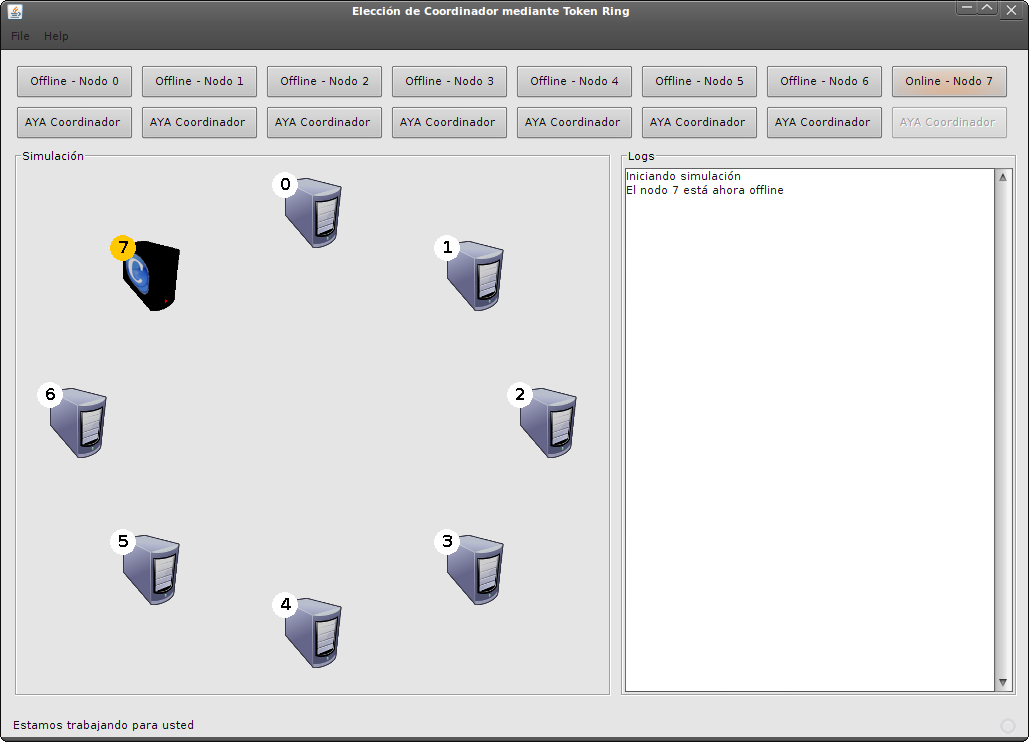
\includegraphics[scale=0.4,keepaspectratio=true]{./imagenes/tokenRing/token1.png}
 \caption{Aqu'i vemos al simulador con el nodo siete caido.}
\end{figure}

\begin{figure}
\centering
 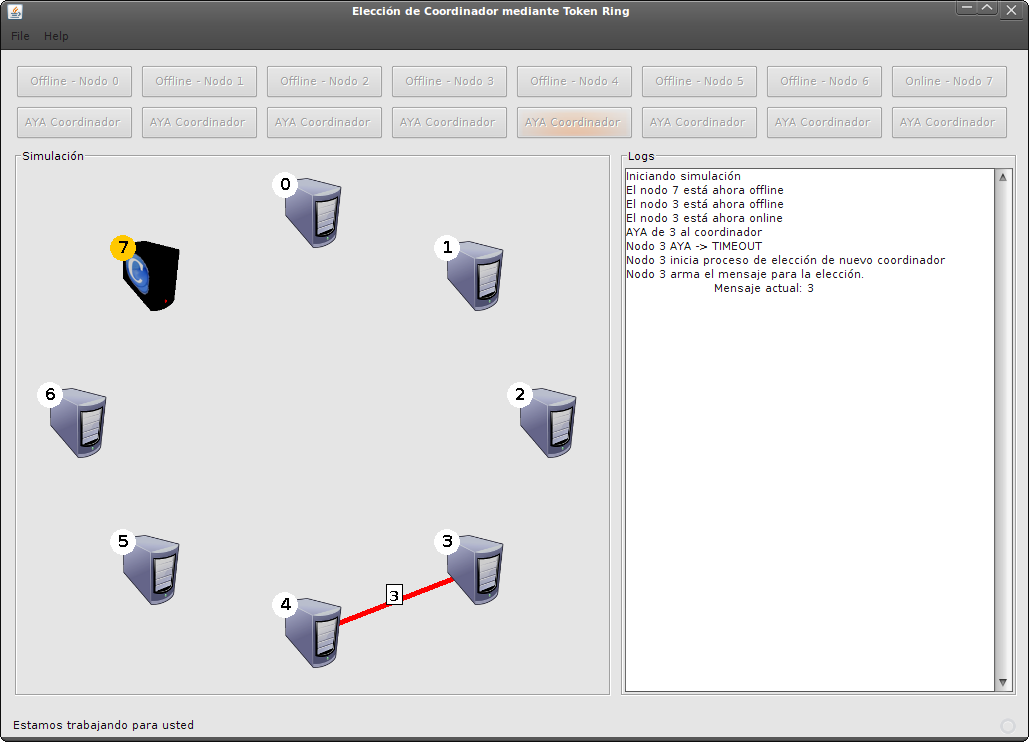
\includegraphics[scale=0.4,keepaspectratio=true]{./imagenes/tokenRing/token2.png}
 \caption{El nodo tres no recibe respuesta del coordinador y comienza el proceso de elecci'on.}
\end{figure}

\begin{figure}
\centering
 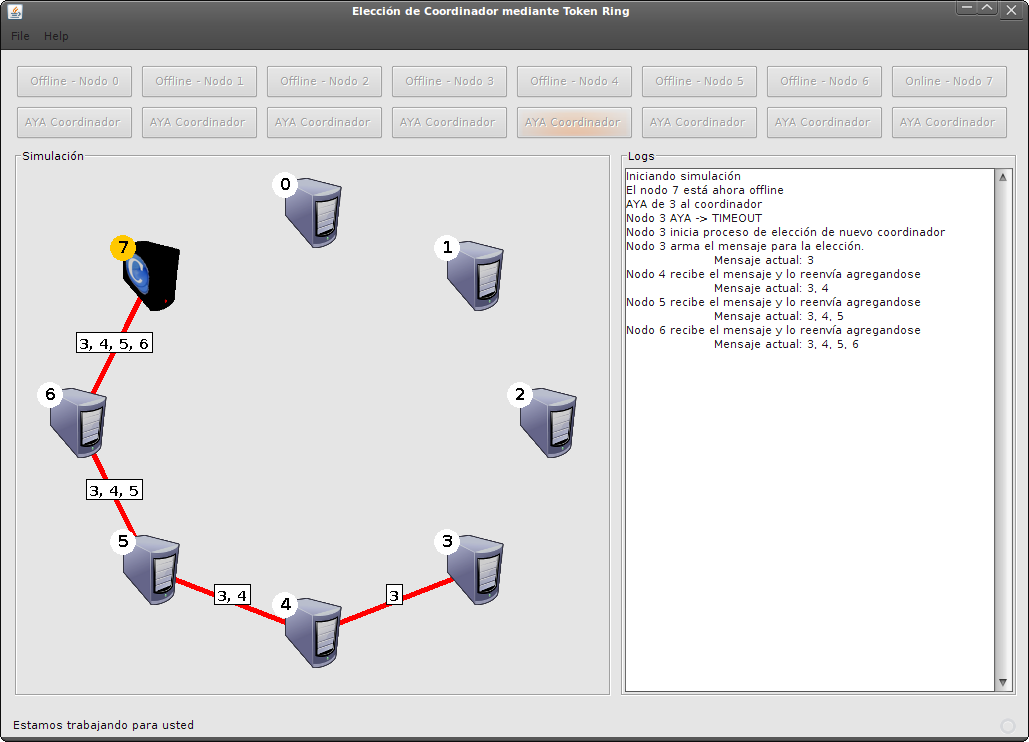
\includegraphics[scale=0.4,keepaspectratio=true]{./imagenes/tokenRing/token3.png}
 \caption{El nodo seis envia un AYA al nodo siete.}
\end{figure}

\begin{figure}
\centering
 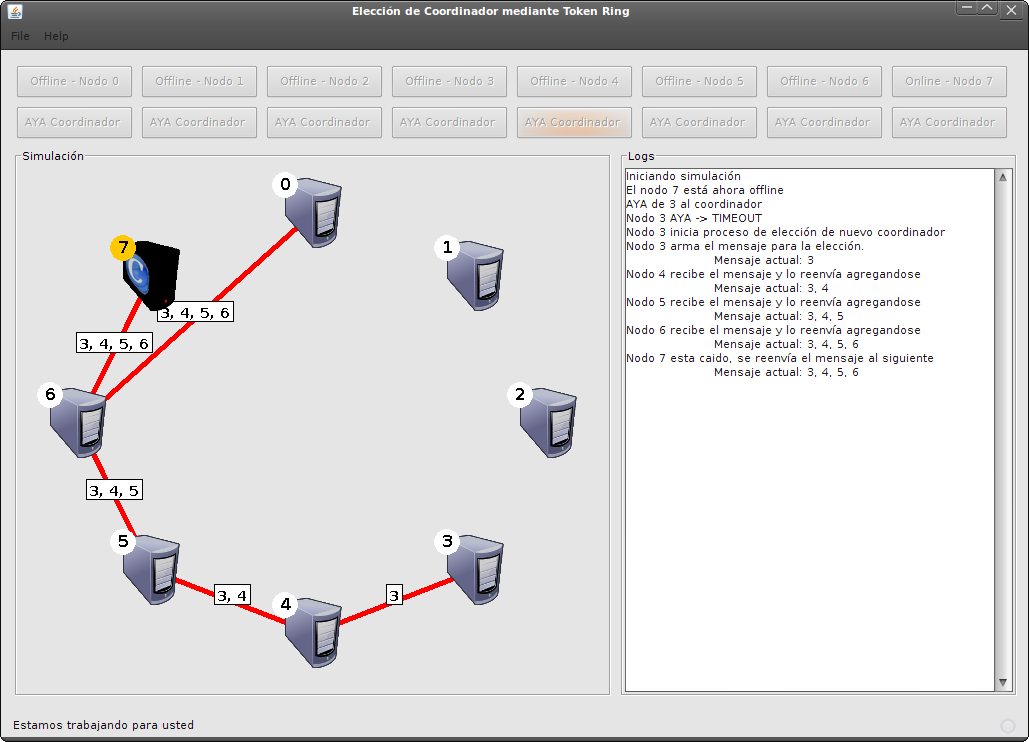
\includegraphics[scale=0.4,keepaspectratio=true]{./imagenes/tokenRing/token4.png}
 \caption{Despu'es de un timeout el nodo seis envia un mensaje de AYA al nodo cero, como este contesta entonces le envia la lista con todos lo nodos activos hasta el momento.}
\end{figure}

\begin{figure}
\centering
 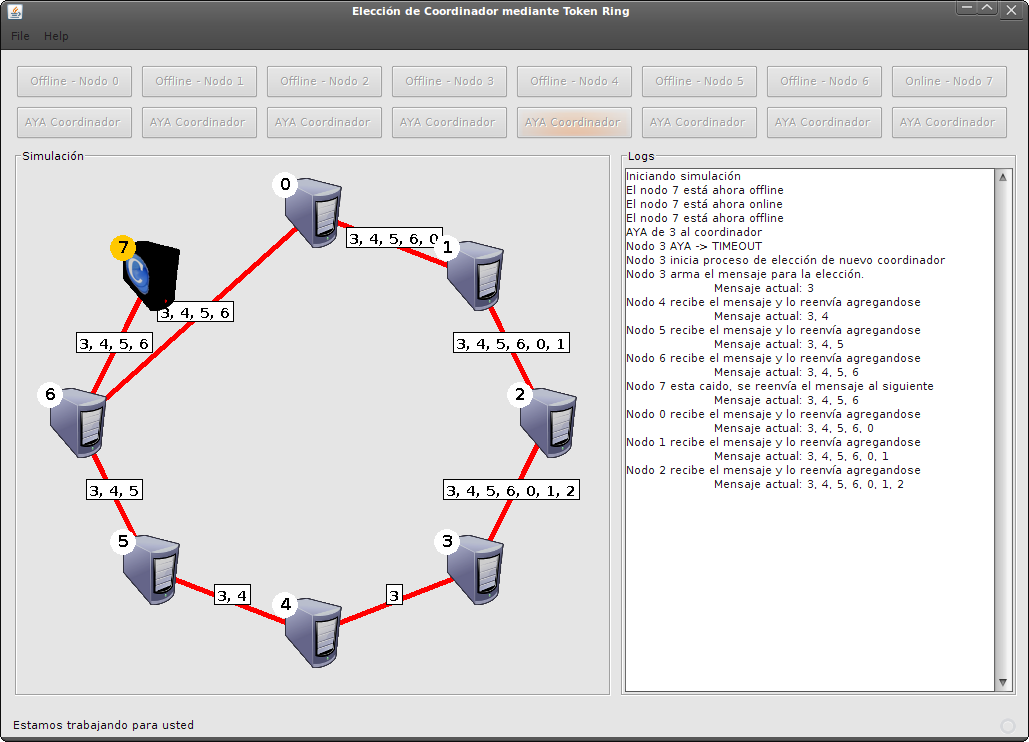
\includegraphics[scale=0.4,keepaspectratio=true]{./imagenes/tokenRing/token5.png}
 \caption{El mensaje termina de pasar por todos los nodos y el nodo tres, selecciona el mayor de los n'umeros en la lista.}
\end{figure}

\begin{figure}
\centering
 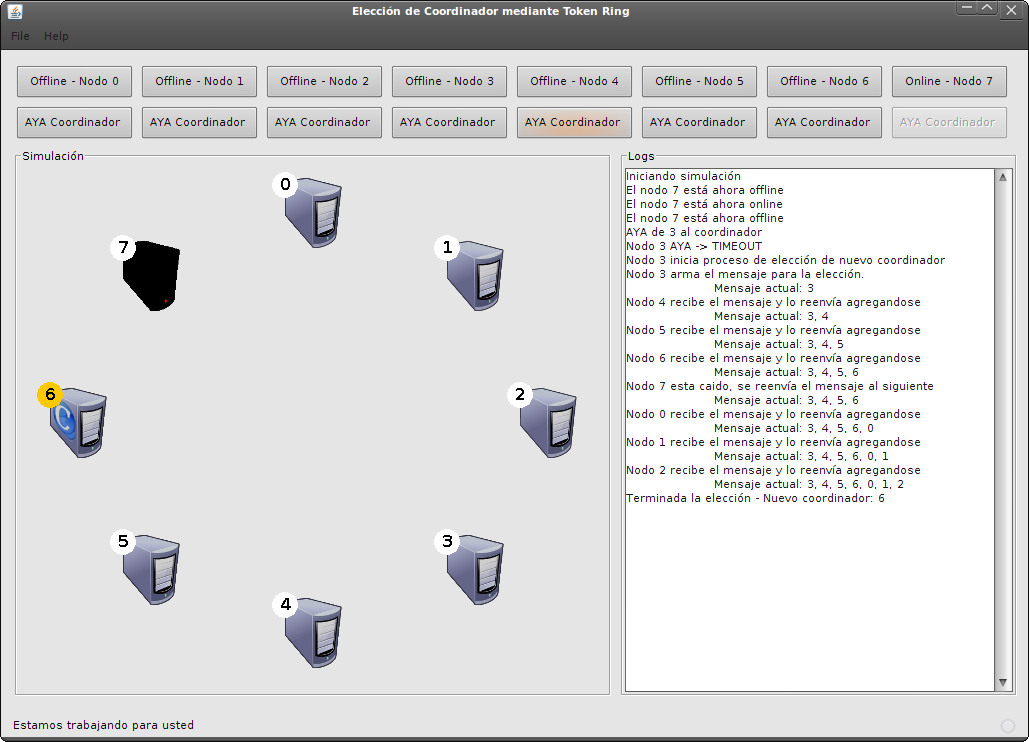
\includegraphics[scale=0.4,keepaspectratio=true]{./imagenes/tokenRing/token6.png}
 \caption{El nodo n'umero tres avisa al resto que el nuevo coordinador es el n'umero seis, este comienza a coordinar al todo el sistema.}
\end{figure}

Veamos un caso en el que m'as de un nodo no responde a los pedidos de los dem'as.

\begin{figure}
\centering
 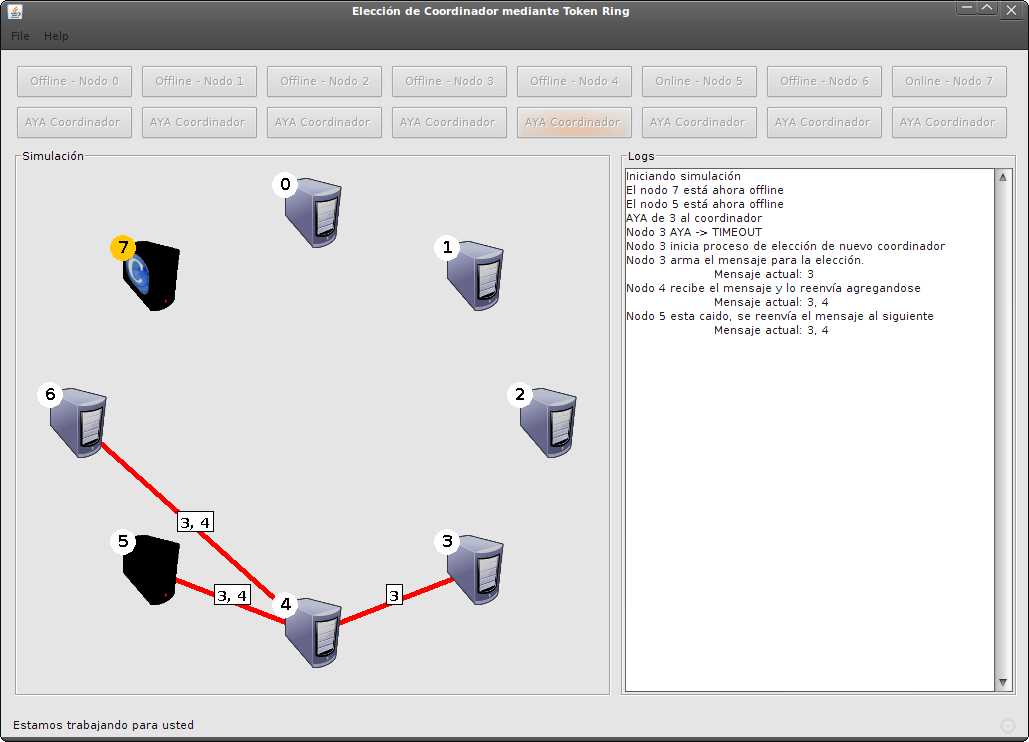
\includegraphics[scale=0.4,keepaspectratio=true]{./imagenes/tokenRing/token7.png}
 \caption{En este caso el nodo siete y el nodo cinco estan caidos, podemos observar como el nodo cuatro envia la lista al nodo seis al determinar que el cinco esta caido.}
\end{figure}

\begin{figure}
\centering
 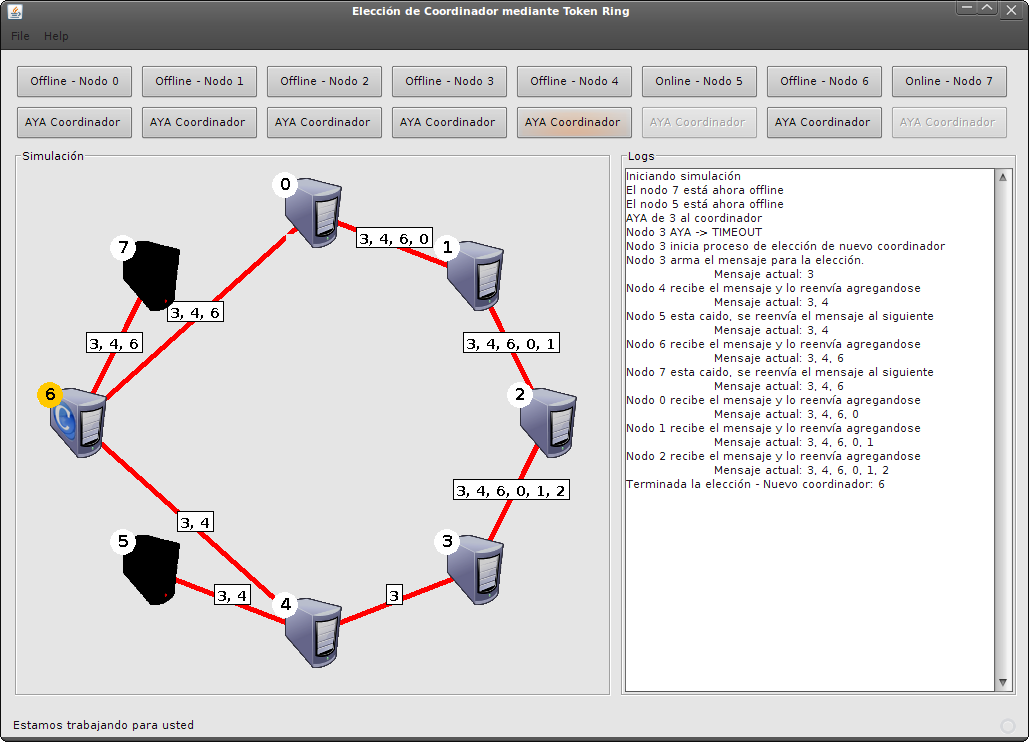
\includegraphics[scale=0.4,keepaspectratio=true]{./imagenes/tokenRing/token8.png}
 \caption{Terminada la elecci'on del nuevo coordinador, podemos observar como el mensaje paso por todos los nodos activos y el nodo seis es el coordinador.}
\end{figure}
